\section{Общая топология}
\begin{definition}
    Топологическим пространством называется упорядоченная пара $(X, \Omega)$, $\Omega \subset 2^X$, причем выполнено 
    \begin{enumerate}
        \item $\emptyset, X \in \Omega$
        \item $\bigcup A_i \in \Omega$ если $\forall i\ A_i \in \Omega$
        \item $\bigcap_{n} A_i \in \Omega$, если $\forall i\ A_i \in \Omega$
    \end{enumerate}
\end{definition}

\begin{definition}
    Связным топологическим пространством называется такое топ. пространство $(X, \Omega)$, в котором нет $A,B \in \Omega$ таких, что $A \cup B = X$ и $A \cap B = \emptyset$.
\end{definition}

\begin{definition}
    Подпространством пространства $(X, \Omega)$ называется топологическое пространство $(X_1, \Omega_1)$, где $X_1 \subset X$ и $\Omega_1 =\{A \cap X_1 \mid A \in \Omega \}$.
    Это подпр-во так же называется индуцированным подпространством.
\end{definition}

\begin{definition}
    Подмножество ($Y$) пр-ва ($(X, \Omega)$) называется связным, если связно индуцированное им подпространство.
\end{definition}

Пример топологии на (подвешенном) лесе.
Теорема: лес связен титт., когда он связен как топ. пространство.

\begin{definition}
    Рассмотрим частично-упорядоченное множество $X$, $(X, \leqslant)$.
    Решеткой называется$\ldots$. 
\end{definition}

Пример: топологическое пространство с порядком по включению является решеткой.
Антипример: произвольное дерево не является решеткой.
\begin{definition}
    Дистрибутивной решеткой называется такая решетка, в которой 
    \[(a+b)c = ac + bc \quad a + bc = (ab)+(ac)  \] 
\end{definition}
(Теорема $\ldots$)

\begin{definition}
    Псевдодополнение $a\to b$ это наибольший $c$ из всех таких $c$, что $ac \leqslant b$.

    Решетка, в которой псевдодополнение определено для всех пар элементов, называется импликативной.
\end{definition}

\begin{figure}
    \begin{center}
        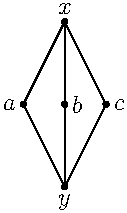
\includegraphics{img/diamont.pdf}
        \caption{Решетка, в которой для $a,b$ не определено псевдодополнение}
    \end{center}
\end{figure}

\begin{definition}
Ноль $0$ и единица $1$~--- это нейтральные элементы операций $+$ и $\cdot$ одновременно.     
\end{definition}

\begin{theorem}
    Рассмотрим импилкативную решетку $(X, \leqslant)$ с 0.
    Рассмотрим интуиционисткое исчисление высказываний, определим оценку следующим образом: 
    $\llbracket \alpha \land \beta \rrbracket = \llbracket \alpha \rrbracket \cdot \llbracket \beta \rrbracket$, $\llbracket \alpha \lor \beta \rrbracket = \llbracket \alpha \rrbracket + \llbracket \beta \rrbracket$, $\llbracket \alpha \to \beta \rrbracket = \llbracket \alpha \rrbracket \to \llbracket \beta \rrbracket$, $\llbracket \neg \alpha \rrbracket = \llbracket \alpha \rrbracket \to 0$.
\end{theorem}

Исчисление высказываний с которым мы работали называется исчислением  гильбертовского типа~--- очень много аксиом и практически одно правило вывода, и это несколько неудобно, как мы увидели.
Не мы одни такие умные. 
Люди придумали что-то ещё.
Полноты ради секвенциальное исчисление будет обсуждаться в конце, если останется время.

Теперь мы обсудим кое-что ещё.
Доказательства в этой системе рисуются в виде дерева, в отличиии от длинного списка, как получается в гильбертовском исчислении.
Вид док-ва: $\Gamma \vdash \varphi$.

Схемы:
\[
    \dfrac{\Gamma, \varphi \vdash \psi}{\Gamma \vdash \varphi \to \psi},~~~
    \dfrac{\Gamma, \varphi \vdash \psi~~~ \Gamma \vdash \varphi}{\Gamma \vdash \psi},~~~
    \dfrac{\Gamma, \varphi ~~~ \Gamma \vdash \psi}{\Gamma \vdash \varphi \& \psi},~~~
    \dfrac{\Gamma, \vdash \varphi \& \psi}{\Gamma \vdash \varphi},~~~
    \dfrac{\Gamma, \vdash \varphi \& \psi}{\Gamma \vdash \psi},
\]\[
    \dfrac{\Gamma \vdash \varphi}{\Gamma\vdash\varphi \vee \psi},~~~
    \dfrac{\Gamma \vdash \psi}{\Gamma\vdash\varphi \vee \psi},~~~
    \dfrac{\Gamma, \varphi \vdash \rho~~~ \Gamma, \psi \vdash \rho~~~ \Gamma \vdash \varphi \vee \psi}{\Gamma\vdash\rho},~~~
    \dfrac{\Gamma \vdash \bot }{\Gamma\vdash\varphi}.
\]
\endinput